% Options for packages loaded elsewhere
\PassOptionsToPackage{unicode}{hyperref}
\PassOptionsToPackage{hyphens}{url}
%
\documentclass[
  man]{apa6}
\usepackage{amsmath,amssymb}
\usepackage{iftex}
\ifPDFTeX
  \usepackage[T1]{fontenc}
  \usepackage[utf8]{inputenc}
  \usepackage{textcomp} % provide euro and other symbols
\else % if luatex or xetex
  \usepackage{unicode-math} % this also loads fontspec
  \defaultfontfeatures{Scale=MatchLowercase}
  \defaultfontfeatures[\rmfamily]{Ligatures=TeX,Scale=1}
\fi
\usepackage{lmodern}
\ifPDFTeX\else
  % xetex/luatex font selection
\fi
% Use upquote if available, for straight quotes in verbatim environments
\IfFileExists{upquote.sty}{\usepackage{upquote}}{}
\IfFileExists{microtype.sty}{% use microtype if available
  \usepackage[]{microtype}
  \UseMicrotypeSet[protrusion]{basicmath} % disable protrusion for tt fonts
}{}
\makeatletter
\@ifundefined{KOMAClassName}{% if non-KOMA class
  \IfFileExists{parskip.sty}{%
    \usepackage{parskip}
  }{% else
    \setlength{\parindent}{0pt}
    \setlength{\parskip}{6pt plus 2pt minus 1pt}}
}{% if KOMA class
  \KOMAoptions{parskip=half}}
\makeatother
\usepackage{xcolor}
\usepackage{graphicx}
\makeatletter
\newsavebox\pandoc@box
\newcommand*\pandocbounded[1]{% scales image to fit in text height/width
  \sbox\pandoc@box{#1}%
  \Gscale@div\@tempa{\textheight}{\dimexpr\ht\pandoc@box+\dp\pandoc@box\relax}%
  \Gscale@div\@tempb{\linewidth}{\wd\pandoc@box}%
  \ifdim\@tempb\p@<\@tempa\p@\let\@tempa\@tempb\fi% select the smaller of both
  \ifdim\@tempa\p@<\p@\scalebox{\@tempa}{\usebox\pandoc@box}%
  \else\usebox{\pandoc@box}%
  \fi%
}
% Set default figure placement to htbp
\def\fps@figure{htbp}
\makeatother
\setlength{\emergencystretch}{3em} % prevent overfull lines
\providecommand{\tightlist}{%
  \setlength{\itemsep}{0pt}\setlength{\parskip}{0pt}}
\setcounter{secnumdepth}{-\maxdimen} % remove section numbering
% Make \paragraph and \subparagraph free-standing
\makeatletter
\ifx\paragraph\undefined\else
  \let\oldparagraph\paragraph
  \renewcommand{\paragraph}{
    \@ifstar
      \xxxParagraphStar
      \xxxParagraphNoStar
  }
  \newcommand{\xxxParagraphStar}[1]{\oldparagraph*{#1}\mbox{}}
  \newcommand{\xxxParagraphNoStar}[1]{\oldparagraph{#1}\mbox{}}
\fi
\ifx\subparagraph\undefined\else
  \let\oldsubparagraph\subparagraph
  \renewcommand{\subparagraph}{
    \@ifstar
      \xxxSubParagraphStar
      \xxxSubParagraphNoStar
  }
  \newcommand{\xxxSubParagraphStar}[1]{\oldsubparagraph*{#1}\mbox{}}
  \newcommand{\xxxSubParagraphNoStar}[1]{\oldsubparagraph{#1}\mbox{}}
\fi
\makeatother
\ifLuaTeX
\usepackage[bidi=basic]{babel}
\else
\usepackage[bidi=default]{babel}
\fi
\babelprovide[main,import]{english}
% get rid of language-specific shorthands (see #6817):
\let\LanguageShortHands\languageshorthands
\def\languageshorthands#1{}
\ifLuaTeX
  \usepackage[english]{selnolig} % disable illegal ligatures
\fi
% Manuscript styling
\usepackage{upgreek}
\captionsetup{font=singlespacing,justification=justified}

% Table formatting
\usepackage{longtable}
\usepackage{lscape}
% \usepackage[counterclockwise]{rotating}   % Landscape page setup for large tables
\usepackage{multirow}		% Table styling
\usepackage{tabularx}		% Control Column width
\usepackage[flushleft]{threeparttable}	% Allows for three part tables with a specified notes section
\usepackage{threeparttablex}            % Lets threeparttable work with longtable

% Create new environments so endfloat can handle them
% \newenvironment{ltable}
%   {\begin{landscape}\centering\begin{threeparttable}}
%   {\end{threeparttable}\end{landscape}}
\newenvironment{lltable}{\begin{landscape}\centering\begin{ThreePartTable}}{\end{ThreePartTable}\end{landscape}}

% Enables adjusting longtable caption width to table width
% Solution found at http://golatex.de/longtable-mit-caption-so-breit-wie-die-tabelle-t15767.html
\makeatletter
\newcommand\LastLTentrywidth{1em}
\newlength\longtablewidth
\setlength{\longtablewidth}{1in}
\newcommand{\getlongtablewidth}{\begingroup \ifcsname LT@\roman{LT@tables}\endcsname \global\longtablewidth=0pt \renewcommand{\LT@entry}[2]{\global\advance\longtablewidth by ##2\relax\gdef\LastLTentrywidth{##2}}\@nameuse{LT@\roman{LT@tables}} \fi \endgroup}

% \setlength{\parindent}{0.5in}
% \setlength{\parskip}{0pt plus 0pt minus 0pt}

% Overwrite redefinition of paragraph and subparagraph by the default LaTeX template
% See https://github.com/crsh/papaja/issues/292
\makeatletter
\renewcommand{\paragraph}{\@startsection{paragraph}{4}{\parindent}%
  {0\baselineskip \@plus 0.2ex \@minus 0.2ex}%
  {-1em}%
  {\normalfont\normalsize\bfseries\itshape\typesectitle}}

\renewcommand{\subparagraph}[1]{\@startsection{subparagraph}{5}{1em}%
  {0\baselineskip \@plus 0.2ex \@minus 0.2ex}%
  {-\z@\relax}%
  {\normalfont\normalsize\itshape\hspace{\parindent}{#1}\textit{\addperi}}{\relax}}
\makeatother

\makeatletter
\usepackage{etoolbox}
\patchcmd{\maketitle}
  {\section{\normalfont\normalsize\abstractname}}
  {\section*{\normalfont\normalsize\abstractname}}
  {}{\typeout{Failed to patch abstract.}}
\patchcmd{\maketitle}
  {\section{\protect\normalfont{\@title}}}
  {\section*{\protect\normalfont{\@title}}}
  {}{\typeout{Failed to patch title.}}
\makeatother

\usepackage{xpatch}
\makeatletter
\xapptocmd\appendix
  {\xapptocmd\section
    {\addcontentsline{toc}{section}{\appendixname\ifoneappendix\else~\theappendix\fi: #1}}
    {}{\InnerPatchFailed}%
  }
{}{\PatchFailed}
\makeatother
\DeclareDelayedFloatFlavor{ThreePartTable}{table}
\DeclareDelayedFloatFlavor{lltable}{table}
\DeclareDelayedFloatFlavor*{longtable}{table}
\makeatletter
\renewcommand{\efloat@iwrite}[1]{\immediate\expandafter\protected@write\csname efloat@post#1\endcsname{}}
\makeatother
\usepackage{lineno}

\linenumbers
\usepackage{csquotes}
\usepackage{bookmark}
\IfFileExists{xurl.sty}{\usepackage{xurl}}{} % add URL line breaks if available
\urlstyle{same}
\hypersetup{
  pdftitle={Time Series Analysis: S\&P 500 Stock Market Closing Prices},
  pdfauthor={Joseph Shin1},
  pdflang={en-EN},
  hidelinks,
  pdfcreator={LaTeX via pandoc}}

\title{Time Series Analysis: S\&P 500 Stock Market Closing Prices}
\author{Joseph Shin\textsuperscript{1}}
\date{}


\shorttitle{Time Series Analysis}

\authornote{

Thank you to all of the support I have received from my professor, TA, and classmates in this course. No matter what result I get from this course, I will always learn from these experiences to develop my work ethic and approach. For this project, I chose to perform a time series analysis on the S\&P 500 Index. I have always wanted to try working with stock market predictions, so I chose to give this an attempt. After completing this project, I have learned a lot through my work, and I plan to grow my skills in the future.

The authors made the following contributions. Joseph Shin: Conceptualization, Writing - Original Draft Preparation, Writing - Review \& Editing, Coding, Interpretations.

}

\affiliation{\vspace{0.5cm}\textsuperscript{1} UIUC}

\abstract{%
In this study, the main objective is to forecast the closing prices of the S\&P 500 stock index using Seasonal Autoregressive Integrated Moving Average, otherwise known as SARIMA. Since stock market prices have a complex pattern influenced by economic factors, investor behavior, market trends, and real-life events, I want to accurately forecast the future closing prices by performing model transformations and model diagnostics to get a more accurate result.

As a result, the next five S\&P 500 closing price predicted values after October 29th, 2024, are \$5,832.61, \$5,832.13, \$5,835.73, \$5,835.73, and \$5,835.73, and the standard error of these values are \$30.48, \$41.59, \$50.67, \$58.26, \$65.00. This result reveals that there is a stable pattern around \$5,832 - \$5,835 for the S\&P 500 stock prices, while the standard errors slowly increases in the future. The fact that the next five forecasted values seems stable rather than showing unexpected fluctuations or continued trends is a surprise. Additionally, even though the standard errors increases, the predicted values are stabilized in a small range of values which emphasizes the confidence in the performance of these values.

Due to the stability, this may imply that the market is much more resilient and the investors are more consistent and confident during this forecasting period. This can mean that the economic conditions are steady, the consumers solidly spend, and the businesses are performing at a consistent pace. Additionally, since the forecast is stable, it may tell investors to not change their current investment strategy. The forecasted S\&P 500 index values suggest market stability, where external influences are balanced, which leads to minimal fluctuations. The increasing uncertainty over time makes sense since as time goes on, since the natural variability may increase as well. This is reflected on the standard errors, and it emphasizes the significance of unpredictability in scientific modeling.
}



\begin{document}
\maketitle

\section{Introduction}\label{introduction}

The problem that I am issuing from this S\&P 500 data set is to determine what the future values of the market's closing price will be after October 29th, 2024. The data provides the daily index value at market close, and the market closing time is at 4 pm ET. The index includes the top 500 leading companies in the leading industries of the U.S. economy, and this covers about 75\% of the U.S. equities. The data shows the market's overall health and trends, which is important for investors, economists, and policymakers in how they make their decisions based on the pattern. The original data set used to have missing dates and values, but I put those missing dates back in and made the values equal to the previous date's closing price value. I also had to change the S\&P 500 observations for the dates that had no information and fill those in with the previous date's closing price value as well.

\url{https://fred.stlouisfed.org/series/SP500\#}

(S\&P Dow Jones Indices LLC)

\section{Methods}\label{methods}

\begin{verbatim}
## Warning: package 'forecast' was built under R version 4.3.3
\end{verbatim}

\begin{verbatim}
## Warning: package 'tseries' was built under R version 4.3.3
\end{verbatim}

\subsection{For my packages, I utilized forecast, tseries, astsa, readr, dplyr, lubridate, and tidyr. To start off, I had to clean the data set first. First, I changed the dates into a date format and filled in the missing dates. Then, for the dates with missing S\&P 500 closing price value, I set those values to the previous day's closing price value.}\label{for-my-packages-i-utilized-forecast-tseries-astsa-readr-dplyr-lubridate-and-tidyr.-to-start-off-i-had-to-clean-the-data-set-first.-first-i-changed-the-dates-into-a-date-format-and-filled-in-the-missing-dates.-then-for-the-dates-with-missing-sp-500-closing-price-value-i-set-those-values-to-the-previous-days-closing-price-value.}

\pandocbounded{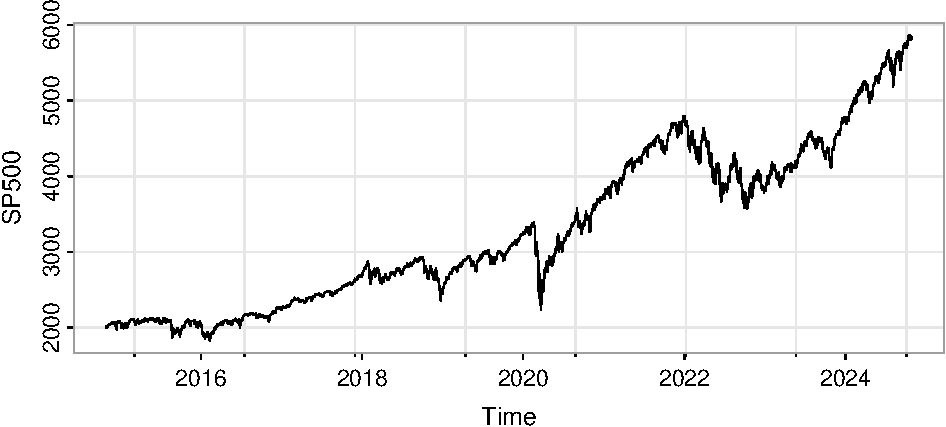
\includegraphics[keepaspectratio]{APATemplate_files/figure-latex/unnamed-chunk-2-1.pdf}}

\begin{verbatim}
## 
##  Augmented Dickey-Fuller Test
## 
## data:  SP500
## Dickey-Fuller = -2.2249, Lag order = 15, p-value = 0.4831
## alternative hypothesis: stationary
\end{verbatim}

Next, I had to make sure my time series was stationary. As you can see in the graph above, it is not stationary. I even tried using the adf.test() function to test the stationarity, and it rejected the null hypothesis since 0.4831 \textgreater{} 0.05 (H0 = Time series is stationary). Therefore, I had to transform the model. The transformation I chose to perform was log-transformation. Additionally, I took the difference of the log transformed model. Here are the results:

\pandocbounded{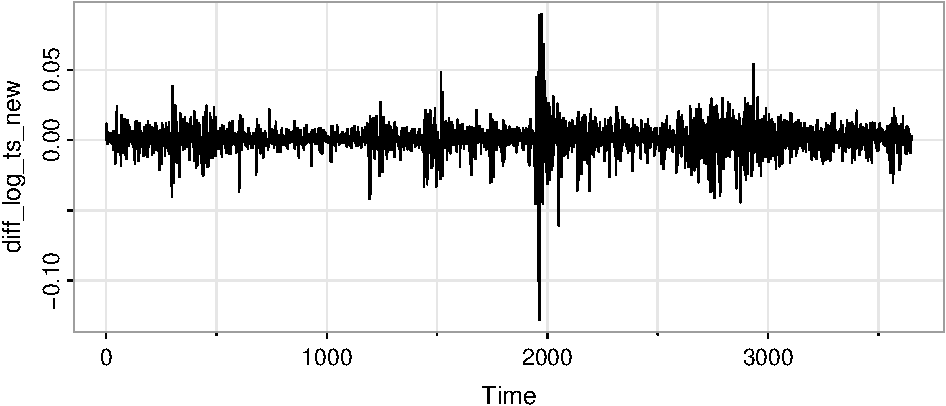
\includegraphics[keepaspectratio]{APATemplate_files/figure-latex/unnamed-chunk-3-1.pdf}}

\begin{verbatim}
## Warning in adf.test(diff_log_ts_new): p-value smaller than printed p-value
\end{verbatim}

\begin{verbatim}
## 
##  Augmented Dickey-Fuller Test
## 
## data:  diff_log_ts_new
## Dickey-Fuller = -14.827, Lag order = 15, p-value = 0.01
## alternative hypothesis: stationary
\end{verbatim}

As you can see in the graph, white noise is present. Additionally, the mean stays constant around a smaller range of values, and the variance does not fluctuate. The adf.test() function also proves that it is stationary since the p-value is smaller than 0.01. Therefore, I chose to continue with this differenced log-transformed model since it was stationary.

\pandocbounded{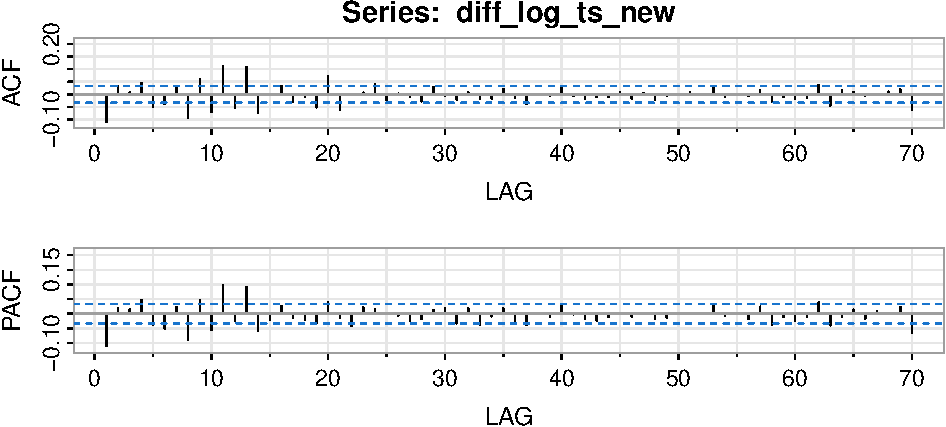
\includegraphics[keepaspectratio]{APATemplate_files/figure-latex/unnamed-chunk-4-1.pdf}}

As you can see in the plots above, the ACF and PACF are both tailing off. This suggests the presence of an ARMA process. Therefore, I tested out multiple different combinations of p, d, q, and seasonal P, D, Q for my sarima function to determine which combination gave the best result.
After testing multiple different models, I narrowed it down to two different models. One of them was where p=1, d=1, q=1, P=0, D=1, and Q=1. The other model consisted of p=1, d=1, q=1, P=1, D=1, and Q=2. For both models, I had to set seasonality equal to 7. I was originally going to set seasonality to 365, but my code kept crashing, so I chose to go for a weekly seasonality using the daily data set instead.

\pandocbounded{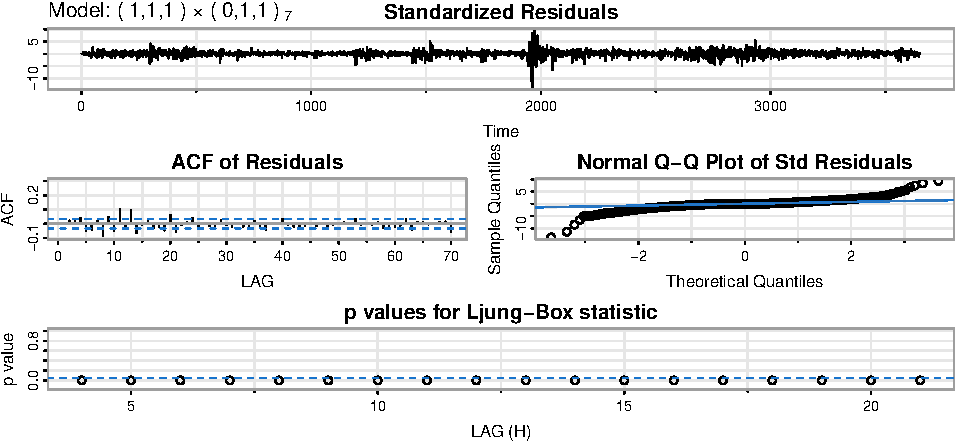
\includegraphics[keepaspectratio]{APATemplate_files/figure-latex/unnamed-chunk-5-1.pdf}} \pandocbounded{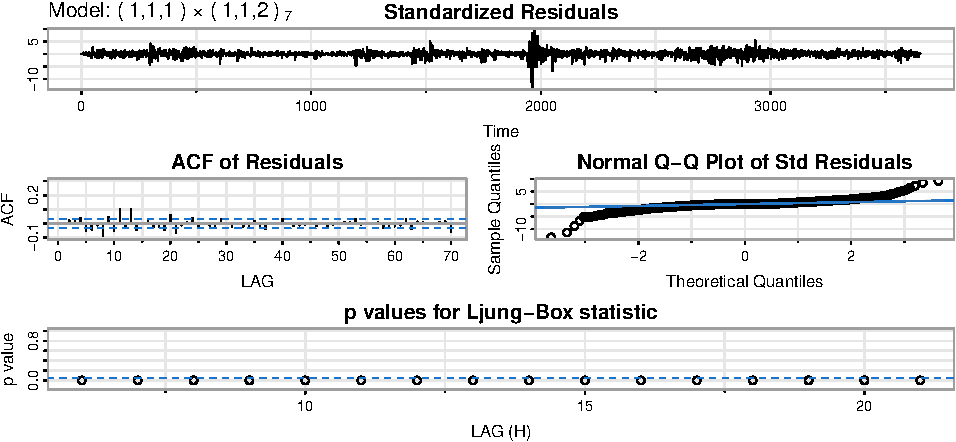
\includegraphics[keepaspectratio]{APATemplate_files/figure-latex/unnamed-chunk-5-2.pdf}}

The reason that these two models were the best model suggestions was because they had the lowest AIC compared to all of the other models I tested. Looking at the summary statistics of these models, they have almost identical results. Because of that, I chose to just commit with one final model, which was snp\_2, since it had a lower AIC compared to snp\_1.

\pandocbounded{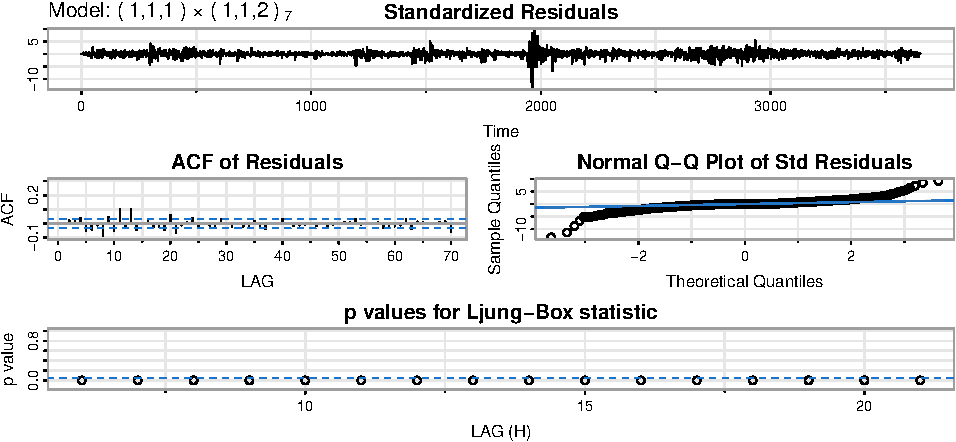
\includegraphics[keepaspectratio]{APATemplate_files/figure-latex/unnamed-chunk-6-1.pdf}}

Based on the standardized residuals plot, there is white noise present, and the residuals are generally centered around zero, which hints that the model is capturing the overall trend.

\section{Results}\label{results}

\pandocbounded{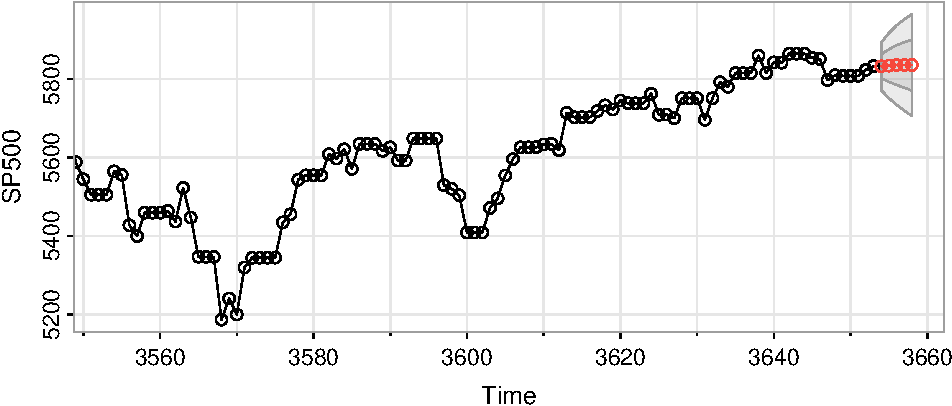
\includegraphics[keepaspectratio]{APATemplate_files/figure-latex/unnamed-chunk-7-1.pdf}}

\begin{verbatim}
## $pred
## Time Series:
## Start = 3654 
## End = 3658 
## Frequency = 1 
## [1] 5832.613 5834.128 5835.730 5835.735 5835.734
## 
## $se
## Time Series:
## Start = 3654 
## End = 3658 
## Frequency = 1 
## [1] 30.47526 41.59328 50.67363 58.26477 64.99951
\end{verbatim}

When performing my forecast, I used the same p, d, q, and seasonal P, D, Q values, but switched to the original dataset because I wanted it to print out the correctly scaled S\&P 500 closing prices. The model's performance captures the trends, especially through short-term forecasts. The confidence intervals give a good idea of what the range of uncertainty is, which is important for investor in how they make their decisions. For stakeholders, it is important for them to not change their methods in how they invest because the values seem to be stabilized during this period. However, the increasing uncertainty confidence interval is something that they should be cautious of since there may be unexpected drops in the stock market.

\section{Discussion}\label{discussion}

Overall, the next five forecasted values of the S\&P 500 daily index of the closing prices are stable. One limitation that my study suffered from was that I had to perform the model with seasonality equal to 7 instead of 365. I think setting the seasonality to 365 would have provided more accurate results. While the model performance went fine, it could benefit from the lack of these limitations.

\newpage

\section{References}\label{references}

S\&P Dow Jones Indices LLC, S\&P 500 {[}SP500{]}, retrieved from FRED, Federal Reserve Bank of St.~Louis; \url{https://fred.stlouisfed.org/series/SP500}, December 20, 2024.

\section{Appendix (Optional)}\label{appendix-optional}

Any R codes or less important R outputs that you wanted to keep- can go in here.


\end{document}
